% !TEX root = ../gnss_interference_resistant_thesis.tex
\documentclass[main.tex]{subfiles}

\begin{document}

\subsection{KerberosSDR laikinės sinchronizacijos matavimas}\label{sec:kerberos_time_sync}

Laikinės sinchronizacijos tikrinimui pasitelktas triukšmų generatorius
integruotas į KerberosSDR imtuvą (aprašyta \ref{sec:kerberossdr} skyriuje).
Signalo užlaikymas skaičiuojamas tokiu pačiu metodu kaip aprašyta \ref{sec:time_sync} skyriuje.

\begin{figure}[h]
    \begin{centering}
    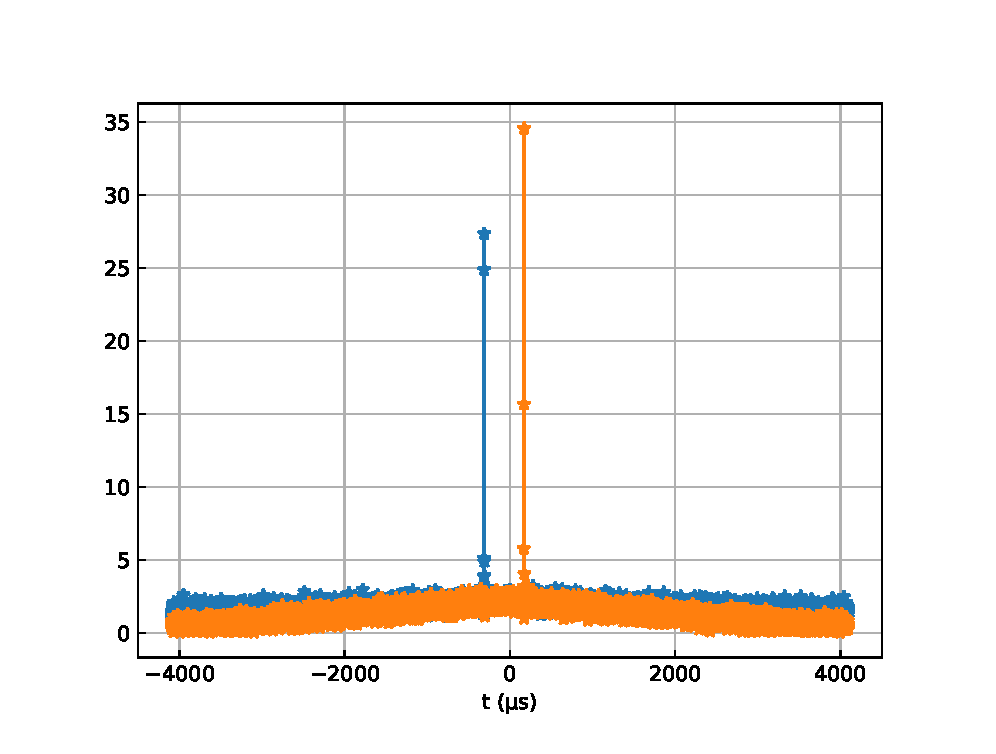
\includegraphics[scale=1.0]{drawings/kerberos_time_sync}
    \par\end{centering}
    \protect\caption{\label{fig:kerberos_timesync}KerberosSDR signalų koreliacijos rezultatas.}
\end{figure}

\ref{fig:kerberos_timesync}~pav. pavaizduota dviejų matavimų rezultatai, tarp kurių imtuvas
buvo inicializuotas iš naujo. Iš grafikų galime matyti, kad vienu atveju signalo
vėlinimas yra $171\ \mathrm{\mu s}$, o kitu $-312\ \mathrm{\mu s}$. Iš šių rezultatų galima
daryti išvada, kad naudojant KerberosSDR imtuvą reikia atlikti taškų vėlinimo kalibravimą.
Priežastys kodėl atsiranda taškų vėlinimas yra tos pačios kaip ir HackRF imtuve, kuris
aprašytas \ref{sec:hackrf} skyriuje.

\end{document}
